% ----------------------------------------------------------------------
\section{Case study: PDPA}\label{sec:case_study_pdpa}

Singapore's Personal Data Protection Act \cite{pdpa_link} consists of a set of
rules governing the use of personal data in private and public organizations,
and describes actions to be taken if a data breach is detected. It consists on
the one hand of \emph{constitutive} rules, \ie{} definitions specifying
what is considered a data breach and under which conditions it is deemed a
notifiable data breach. On the other hand, \emph{regulative} rules prescribe
which actions need to be taken if a notifiable data breach is detected.

The constitutive rules are sufficiently voluminous and complex to warrant the
development of an expert system assisting organizations in assessing whether a
data breach is notifiable. In the CCLAW project, we have developed such a
system, which is described \remms{elsewhere. Reference?}. The regulative rules
are seemingly less involved but sufficiently intricate that actors that
precisely follow the rules may wind up in a state where they have breached the
law. The complexity results from the interplay of temporal conditions that
remain implicit and that would have to be explicated to guarantee lawful
behavior.

We here give an abridged account of the relevant rules; for details, see
\S\S~26A to E of \cite{pdpa_link} that leads to and motivates our
formalization in \secref{sec:formal_analysis}. The PDPA identifies three
actors in a data breach scenario:
\begin{itemize}
\item the \emph{organization} in which a data breach has occurred;
\item the Personal Data Protection Commission (PDPC, henceforth only called
  the \emph{commission}), the governmental authority that has to be notified
  in case of a breach;
\item the \emph{individual} affected by a data breach. The abstraction of the
  multitude of affected individuals to a single entity is already done in the
  law text and seems appropriate as there is no interaction among the
  individuals. 
\end{itemize}

The temporal requirements are as follows:
\begin{itemize}
\item When a data breach is detected, the organization has up to thirty days to
  assess whether the data breach is notifiable; if it is not, no further
  action is required, and the process stops there. 
\item If the breach is notifiable, the organization is obliged to inform the
  commission within three days of having recognized the breach as notifiable.
\item If the breach is notifiable, any affected individual also has to be
  informed within the three day period.
\item The organization must not notify an affected individual if the
  commission so directs.
\end{itemize}

The inconsistency, that was in part revealed by the formalization and then
confirmed by model checking, arises from the lack of temporal coordination
between the action of informing the commission and the individual, and
possibly the interdiction by the commission to inform the individual.


%----------------------------------------------------------------------
\section{Formal Analysis}\label{sec:formal_analysis}

We have carried out a formal analysis of this scenario with the Uppaal
\cite{larsen1997uppaal} model checker. The global setup is shown in
\figref{fig:pdpa}. There are three interacting automata, one for each of the
above-mentioned actors. The states carry names (in mauve), the initial states
are marked with a double circle. The automata synchronize via messages (in
turquoise), where a send action is indicated by an exclamation and a receive
action by a question mark. Transitions may depend on Boolean conditions (here:
variables such as \texttt{isNotifiable}) and on temporal conditions modeled
with the aid of \emph{clocks}. In this example, there is one closk,
\texttt{cl}, that is zero in the initial state, and that is again reset to
zero in the transition from \texttt{breachDetected} to \texttt{breachDeterminedNotifiable}.


\begin{figure}[htp]
\centering
\subfloat[Commission\label{fig:commission}]{%
  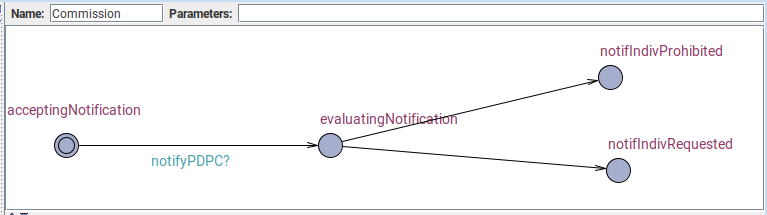
\includegraphics[width=0.65\textwidth]{Figures/commission.png}%
}\hfil
\subfloat[Individual\label{fig:individual}]{%
  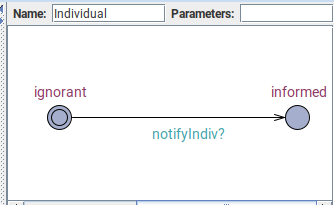
\includegraphics[width=0.3\textwidth]{Figures/individual.png}%
}\\
\subfloat[Organization\label{fig:organization}]{%
  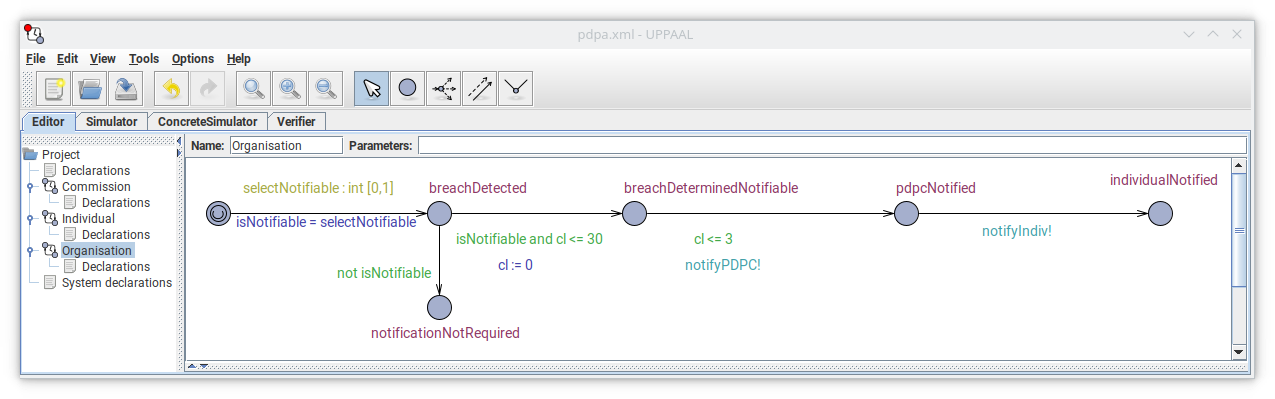
\includegraphics[width=\textwidth]{Figures/organization.png}%
}
\caption{Automata modelling the PDPA scenario}
\label{fig:pdpa}
\end{figure}


\begin{itemize}
\item Original formal analysis with race condition
\item Introducing deadlines for feedback by the commission. If the feedback deadline is
  sufficiently close to the deadline for informing the individual, the law may
  not be formally inconsistent, but the process is not \emph{realizable} any
  more for a real organization.
\end{itemize}

%----------------------------------------------------------------------
\section{Modularization}



%%% Local Variables:
%%% mode: latex
%%% TeX-master: "main"
%%% End:
